\begin{letter}{2}
\begin{header}
\from{Weyl}
\to{Pauli}
\date{1919/12/09}
\location{Zurich}

\makeheader

\end{header}

Very honorable Herr Pauli!

Many thanks for the \?{proofs}{Korrekturbogen} and your paper from the Physikalische Zeitschrift! Please don't take my silence too badly. Written correspondence with people is grueling for me; lately I have been with completely different things, logical foundations of analysis, and am impeded by shaky health.

Regarding your result that the Einstein field of a "point mass" is also a rigorous solution of the field equations associated with the action quantities $R_{iklm}^{iklm}$, I am naturally pleased. — I likewise find the \?{over-determination}{Überbestimmtheit} of the static field more pleasant than alarming. I find that only the \textit{static, spherically-symmetric} has a physical meaning (an actually static solution can only be spherically symmetric), and so the over-determination vanishes. It seems to me that nothing else is to be expected with rigorous field equations. The essential difference between the two electricities can emerge in Mie's theory via a root, e.g. $\sqrt{\varphi_i \varphi_i}$ in this way: if there are any roots in the static case, according to the principle of analytic continuation, $\varphi_0$ \textit{and not $=|\varphi_0|$} (I assume $ds^2 = dx_0^2 - dx_1^2 - dx_2^2 - dx_3^2$). In a non-static field deviating little from that, it is impossible for $\varphi_i\varphi^i >0$ everywhere; that must be discussed in more detail. In any cade, with many-valued functions in the action principle a single analytic branch among these is understood, the selection of which \textit{cannot} be done in a coordinate-free manner. Why should that be excluded in my theory? But we are now ignoring just such a many-valuedness! If we have an isolated system that sweeps out a world-tube, then its charge $e$ equals the flux of the vector density $\mathcal{E}_i$ through an arbitrary cross-section $S$ of the tube:

%\fig{02-19191209-01}

\begin{figure}[h]
	\begin{center}
	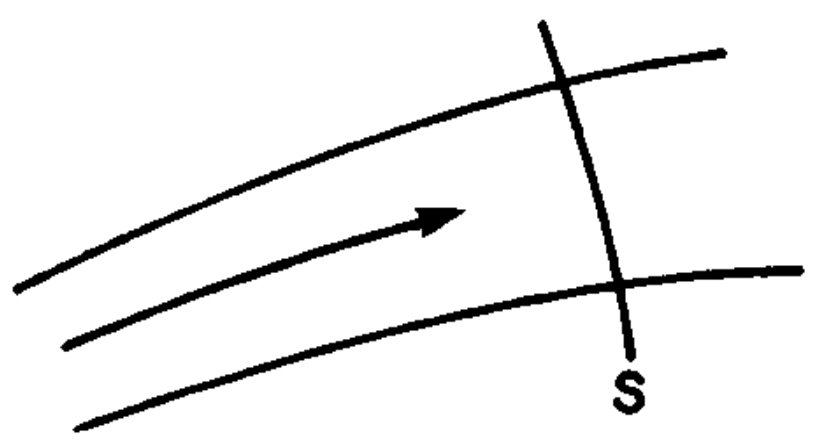
\includegraphics[width=150pt]{02-19191209-01}
	\end{center}
\end{figure}

$e$ is an absolutely definite number as soon as a flow direction (past $\to$ future) is fixed in the tube. That is what I meant with my assertion that the sign of the charge is dependent on the distinction between past and future. I hold, as opposed to most physicists, their essential difference to be a fact of much more fundamental significance than the essential difference between positive and negative electricity. Nevertheless, modern physics is right that it has no place in "laws" or "field physics". \?{I am then firmly convinced that statistics are fundamentally independent with regards to causality, which is a "law"; while it is just absurd to suppose a continuum as something pre-existing}{Denn ich bin fest überzeugt davon, daß die Statistik etwas prinzipiell selbstständiges gegenüber der Kausalitat, dem "Gesetz" ist; weil es übberhaupt widersinnig ist, sich ein Kontinuum als etwas fertig-Seiendes vorzustellen}. Field theory, I think, really only plays the role of "world geometry"; in matter there is still something else, something real, that is not causally interpretable, but rather perhaps can be thought of under the concept "independent decisions", and which we treat in physics through statistical calculations. It is quite possible that we must must leave the essential distinction between past and future, between positive and negative electricity here; that it will then still find no place in field theory. These are \textit{suggestions} whose more detailed investigation would take too much space.

I am in agreement with you that the legitimacy of speaking of a conservation law $\pXpY{\gamma_i^k}{x_k} = 0$ as an energy-momentum law must be disproven by the fact that for a material particle it yields the mechanical equations. Your derivation of the same shared in your last letter however did not seem as compelling to me.

That the fields inside the electron cannot be measured, one can probably only say: differences inside the electron could never \?{causally create}{kausal bedingen} such changes in the course of the world which grow to an immediately-perceptible magnitudes. Namely, as soon as such effects occur, I can use them to "measure" any interior differences. But why should that not happen! I believe e.g. that the circumstance that electron does not radiate in the stationary Bohr orbits, is a sign of an inner change in the electron arising through the acceleration that allows it to keep its energy; then why should it behave like a rigid sphere with rigid charge even with non-quantized acceleration?

With best thanks and greetings, yours faithfully

H. Weyl



\end{letter}
